\documentclass{article}
%Usepackages
\usepackage{adjustbox, amsmath, amssymb, amsthm, blindtext, bm, bbm, dblfloatfix, esint, fancyhdr, float, graphicx, letltxmacro, marginnote, mathtools, subcaption, xcolor, titlesec, esint}
\usepackage{amssymb}
\usepackage[font={small, it}]{caption}
\usepackage{amsmath}
\usepackage{floatrow}
\usepackage{times}
\usepackage{ stmaryrd }
\usepackage{amsthm}
\usepackage{xcolor}
\usepackage{mathrsfs}
\usepackage[colorlinks = true,
            linkcolor = black,
            urlcolor  = blue,
            citecolor = black,
            anchorcolor = blue]{hyperref}
% \usepackage[mathscr]{euscript}
\usepackage{mathrsfs}
\usepackage{wasysym}
%\usepackage{pxfonts}
\usepackage[letterpaper, portrait, margin=1in]{geometry}
\usepackage{graphicx}
\usepackage{tikz}
\usepackage{tikz-3dplot}
\usepackage{pgfplots}
\usetikzlibrary{decorations.pathmorphing,patterns}
\usepackage{lipsum}
\usepackage{float}
\usepackage{subcaption}
\usepackage[object=vectorian]{pgfornament}
\usepackage{mwe}
\usepackage{bigints}
\usepackage{csquotes}
\usepackage{titlesec}
\usepackage{halloweenmath}
\setcounter{secnumdepth}{4}
\titleformat{\paragraph}
{\normalfont\normalsize\bfseries}{\theparagraph}{1em}{}
\titlespacing*{\paragraph}
{0pt}{3.25ex plus 1ex minus .2ex}{1.5ex plus .2ex}
\usepackage{mathtools}
\usepackage{pgfplots}
\pgfplotsset{compat=1.15}
\usepackage{lastpage}
\usepackage{enumitem}
\usepackage{tensor}
\usepackage{mathtools}

% This is for the header:
% https://tex.stackexchange.com/questions/75168/get-current-section-name-without-label
\usepackage{nameref}
\makeatletter
\newcommand*{\currentname}{\@currentlabelname}
\makeatother

\usepackage{fancyhdr} 
    \pagestyle{fancy}
    \fancyhf{}
    \fancyhead[R]{ Page \thepage \  of \pageref{LastPage}}
    \fancyhead[L]{\currentname}
\usepackage{setspace}
\usepackage{tikz}
\usetikzlibrary{hobby}

\usepackage{pst-node}
\usepackage{tikz-cd}
\usepackage[most]{tcolorbox}

% \makeatletter
% \renewcommand\@endtheorem{\vvv@endmarker\endtrivlist\@endpefalse}
% \newcommand\vvv@endmarker{%
%   {\unskip\nobreak\hfil\penalty50
%   \hskip2em\vadjust{}\nobreak\hfil\openbox
%   \parfillskip=0pt \finalhyphendemerits=0 \par
%   \penalty 10000 \parskip=0pt\noindent}\ignorespaces}
% \makeatother

\theoremstyle{definition}

% https://tex.stackexchange.com/questions/616586/how-to-make-a-tcolorbox-with-only-a-left-side-rule


\newtheorem{thm}{Theorem}[section]
\newtheorem{defn}[thm]{Definition}
\newtheorem{exmp}[thm]{Example}
\newtheorem{lem}[thm]{Lemma}
\newtheorem{conjecture}[thm]{Conjecture}
\newtheorem{exercise}[thm]{Exercise}
\newtheorem{fact}[thm]{Fact}
\newtheorem{claim}[thm]{Claim}
\newtheorem{cor}[thm]{Corollary}
\newtheorem{summary}[thm]{Summary}

\newtheorem{idea}[thm]{Idea}
\newtheorem{application}[thm]{Application}
\newtheorem{rmk}[thm]{Remark}

\newtheorem{prop}[thm]{Proposition}
\newtheorem{ques}[thm]{Question}
\newtheorem{observation}[thm]{Observation}

\newtcolorbox{cbox}[1][]{
            breakable,
            boxrule=0pt,
            frame hidden,
            sharp corners,
            enhanced,
            borderline west={2pt}{0pt}{#1},
            colback=#1!5!white}

% \newenvironment{cthm}[3]
%     {\begin{cbox}[#2]
%     \color{#2}
%     \begin{#3}[#1]
%     \color{black}
%     }
%     {
%     \end{#3} 
%     \end{cbox}
%     }

% \newenvironment{theorem}[1][]
% {\begin{cthm}{#1}{orange}{thm}}
% {\end{cthm}}

\newenvironment{theorem}[1][]
    {\begin{cbox}[blue]
    \color{blue}
    \begin{thm}[#1]
    \color{black}
    }
    {
    \end{thm} 
    \end{cbox}
    }

\newenvironment{corollary}[1][]
    {\begin{cbox}[orange]
    \color{orange}
    \begin{cor}[#1]
    \color{black}
    }
    {
    \end{cor} 
    \end{cbox}
    }

\newenvironment{lemma}[1][]
    {\begin{cbox}[orange]
    \color{orange}
    \begin{lem}[#1]
    \color{black}
    }
    {
    \end{lem} 
    \end{cbox}
    }

\newenvironment{proposition}[1][]
    {\begin{cbox}[orange]
    \color{orange}
    \begin{prop}[#1]
    \color{black}
    }
    {
    \end{prop} 
    \end{cbox}
    }

\newenvironment{definition}[1][]
    {\begin{cbox}[red]
    \color{red}
    \begin{defn}[#1]
    \color{black}
    }
    {
    \end{defn} 
    \end{cbox}
    }

\newenvironment{example}[1][]
    {\begin{cbox}[violet]
    \color{violet}
    \begin{exmp}[#1] \color{black}
    }
    {
    \end{exmp} 
    \end{cbox}
    }

\newenvironment{question}[1][]
    {\begin{cbox}[black]
    \begin{ques}[#1]
    }
    {
    \end{ques} 
    \end{cbox}
    }

\newenvironment{remark}[1][]
    {\begin{cbox}[black]
    \begin{rmk}[#1]
    }
    {
    \end{rmk} 
    \end{cbox}
    }



\newenvironment{solution}
  {\renewcommand\qedsymbol{$\blacksquare$}\begin{proof}[Solution]}
  {\end{proof}}
\newenvironment{answer}
  {\begin{proof}[Answer]}
  {\end{proof}}
  
% \newenvironment{example}
%   {\pushQED{\qed}\renewcommand{\qedsymbol}{$\triangle$}\examplex}
%   {\popQED\endexamplex}


%%%%%%%%%%%%%%%%%%%%%%%%%%%%%

%Custom Commands
    \renewcommand\qedsymbol{$\blacksquare$}
    \newcommand{\Pcal}{\mathcal{P}}
    \newcommand{\ve}{\varepsilon}
    \newcommand{\Ocal}{\mathcal{O}}
    \newcommand{\Asf}{\textsf{A}}
    \newcommand{\al}{\alpha}
    \newcommand{\be}{\beta}
    \newcommand{\Nbb}{\mathbb{N}}
    \newcommand{\Si}{\Sigma}
    \newcommand{\Hbb}{\mathbb{H}}
    \DeclareMathOperator{\diag}{diag}
    \newcommand{\De}{\Delta}
    \newcommand{\Xcal}{\mathcal{X}}
    \newcommand{\si}{\sigma}
    \newcommand{\Ga}{\Gamma}
    \newcommand{\Cscr}{\mathscr{C}}
    \newcommand{\1}{\mathbf{1}}
    \newcommand{\Dcal}{\mathcal{D}}
    \newcommand{\Iscr}{\mathscr{I}}
    \newcommand{\Pbb}{\mathbb{P}}
    \newcommand{\B}{\mathbb{B}}
    \newcommand{\Dscr}{\mathscr{D}}
    \newcommand{\Nfrak}{\mathfrak{N}}
    \newcommand{\Efrak}{\mathfrak{E}}
    \DeclareMathOperator{\charp}{charpoly}
    \newcommand{\Csf}{\mathsf{C}}
    \newcommand{\rfrak}{\mathfrak{r}}
    \newcommand{\Sbb}{\mathbb{S}}
    \newcommand{\La}{\Lambda}
    \newcommand{\de}{\delta}
    \DeclareMathOperator{\inte}{int}
    \DeclareMathOperator{\ord}{ord}
    \newcommand{\set}{\mathsf{set}}
    \newcommand{\Bscr}{\mathscr{B}}
    \newcommand{\Zscr}{\mathscr{Z}}
    \newcommand{\ab}{\mathrm{ab}}
    \newcommand{\Xscr}{\mathscr{X}}
    \newcommand{\Escr}{\mathscr{E}}
    \newcommand{\Gscr}{\mathscr{G}}
    \DeclareMathOperator{\Sym}{Sym}
    \newcommand{\om}{\omega}
    \newcommand{\gfrak}{\mathfrak{g}}
    \newcommand{\hfrak}{\mathfrak{h}}
    \newcommand{\kfrak}{\mathfrak{k}}
    \newcommand{\Grp}{\mathsf{Grp}}
    \newcommand{\Ab}{\mathsf{Ab}}
    \newcommand{\xbar}{\bar{x}}
    \newcommand{\abar}{\bar{a}}
    \newcommand{\ybar}{\bar{y}}
    \DeclareMathOperator{\coker}{coker}
    \newcommand{\Modsf}{\mathsf{Mod}}
    \newcommand{\op}{\mathrm{op}}
    \newcommand{\Ring}{\mathsf{Ring}}
    \newcommand{\modsf}{\mathsf{mod}}
    \DeclareMathOperator{\Alt}{Alt}
    \newcommand{\Om}{\Omega}
    \newcommand{\ze}{\zeta}
    \newcommand{\Fcal}{\mathcal{F}}
    \newcommand{\Oscr}{\mathscr{O}}
    \newcommand{\gl}{\mathfrak{gl}}
    \DeclareMathOperator{\Lie}{Lie}
    \DeclareMathOperator{\GL}{GL}
    \DeclareMathOperator{\SL}{SL}
    \DeclareMathOperator{\Vol}{Vol}
    \DeclareMathOperator{\Disc}{Disc}
    \DeclareMathOperator{\SO}{SO}
    \newcommand{\Xfrak}{\mathfrak{X}}
    \DeclareMathOperator{\id}{id}
    \DeclareMathOperator{\Int}{Int}
    \DeclareMathOperator{\End}{End}
    \DeclareMathOperator{\Aut}{Aut}
    \DeclareMathOperator{\stab}{stab}
    \DeclareMathOperator{\orb}{orb}
    \DeclareMathOperator{\grad}{grad}
    \DeclareMathOperator{\curl}{curl}
    \newcommand{\vp}{\varphi}
    \newcommand{\vt}{\vartheta}
    \DeclareMathOperator{\Gal}{Gal}
    \DeclareMathOperator{\rank}{rank}
    \DeclareMathOperator{\col}{col}
    \DeclareMathOperator{\Tame}{Tame}  
    \newcommand{\Yscr}{\mathscr{Y}}
    \newcommand{\Fbb}{\mathbb{F}}
    \newcommand{\Hcal}{\mathcal{H}}
    \newcommand{\arctanh}{\text{arctanh}}
    \newcommand{\pa}{\partial}
    \newcommand{\del}{\boldsymbol{\nabla}}
    \newcommand{\na}{\nabla}
    \newcommand{\Ycal}{\mathcal{Y}}
    \DeclareMathOperator{\spn}{span}
    \DeclareMathOperator{\Inn}{Inn}
    \DeclareMathOperator{\chara}{char}
    \newcommand{\lap}{\nabla^2}
    \newcommand{\Pfrak}{\mathfrak{P}}
    \newcommand{\mfrak}{\mathfrak{m}}
    \newcommand{\Fvec}{\mathbf{F}}
    \newcommand{\Mcal}{\mathcal{M}}
    \newcommand{\ellvec}{\boldsymbol{\ell}}
    \newcommand{\rvec}{\mathbf{r}}
    \DeclareMathOperator{\supp}{supp}
    \newcommand{\Abb}{\mathbb{A}}
    \newcommand{\svec}{\mathbf{s}}
    \newcommand{\VECT}{\mathsf{VECT}}
    \newcommand{\fs}{\vec{\sigma}}
    \newcommand{\bs}{\cev{\sigma}}
    \newcommand{\uvec}{\mathbf{u}}
    \newcommand{\iunit}{\boldsymbol{\hat{\i}}}
    \newcommand{\junit}{\boldsymbol{\hat{\j}}}
    \newcommand{\xunit}{\mathbf{\hat{x}}}
    \newcommand{\Char}{\text{char}}
    \newcommand{\kunit}{\mathbf{\hat{k}}}
    \newcommand{\theunit}{\boldsymbol{\hat{\theta}}}
    \newcommand{\pvec}{\mathbf{p}}
    \newcommand{\qvec}{\mathbf{q}}
    \newcommand{\Qcal}{\mathcal{Q}}
    \newcommand{\yvec}{\mathbf{y}}
    \newcommand{\xvec}{\mathbf{x}}
    \newcommand{\wvec}{\mathbf{w}}
    \newcommand{\bvec}{\mathbf{b}}
    \newcommand{\Ucal}{\mathcal{U}}
    \newcommand{\Ncal}{\mathcal{N}}
    \newcommand{\Scal}{\mathcal{S}}
    \newcommand{\Nscr}{\mathscr{N}}
    \newcommand{\da}{\dagger}
    \newcommand{\CT}{\mathrm{H}}
    \newcommand{\Sscr}{\mathscr{S}}
    \DeclareMathOperator{\lcm}{lcm}
    \newcommand{\evec}{\mathbf{e}}
    \newcommand{\Kscr}{\mathscr{K}}
    \newcommand{\ebold}{\boldsymbol{e}}
    \newcommand{\zvec}{\mathbf{z}}
    \newcommand{\vvec}{\mathbf{v}}
    \newcommand{\Tscr}{\mathscr{T}}
    \newcommand{\avec}{\mathbf{a}}
    \newcommand{\Avec}{\mathbf{A}}
    \newcommand{\Ivec}{\mathbf{I}}
    \newcommand{\ivec}{\mathbf{i}}
    \newcommand{\jvec}{\mathbf{j}}
    \newcommand{\kvec}{\mathbf{k}}
    \newcommand{\of}{\mathfrak{o}}
    \DeclareMathOperator{\Ot}{O}
    \DeclareMathOperator{\Sy}{S}
    \newcommand{\slf}{\mathfrak{sl}}
    \newcommand{\muvec}{\boldsymbol{\mu}}
    \newcommand{\Bvec}{\mathbf{B}}
    \newcommand{\Cvec}{\mathbf{C}}
    \newcommand{\eunit}{\mathbf{\hat{e}}}
    \newcommand{\vpunit}{\boldsymbol{\hat{\varphi}}}
    \newcommand{\zero}{\boldsymbol{0}}
    \newcommand{\tauvec}{\boldsymbol{\tau}}
    \newcommand{\runit}{\mathbf{\hat{r}}}
    \newcommand{\U}{\mathcal{U}}
    \newcommand{\Zbb}{\mathbb{Z}}
    \newcommand{\Dbb}{\mathbb{D}}
    \newcommand{\Bsf}{\mathsf{B}}
    \DeclareMathOperator{\G}{G}
    \newcommand{\gmat}{\textsf{g}}
    \newcommand{\Ccal}{\mathcal{C}}
    \newcommand{\SM}{\mathsf{SM}}
    \newcommand{\VB}{\mathsf{VB}}
    \newcommand{\Dsf}{\mathsf{D}}
    \newcommand{\Fscr}{\mathscr{F}}
    \DeclareMathOperator{\Map}{Map}
    \DeclareMathOperator{\Frob}{Frob}
    \newcommand{\Imat}{\textsf{I}}
    \newcommand{\Rmat}{\textsf{R}}
    \DeclareMathOperator{\Frac}{Frac}
    \DeclareMathOperator{\Spec}{Spec}
    \DeclareMathOperator{\Emb}{Emb}
    \newcommand{\Kcal}{\mathcal{K}}
    \newcommand{\Wcal}{\mathcal{W}}
    \newcommand{\Lcal}{\mathcal{L}}
    \newcommand{\Tcal}{\mathcal{T}}
    \newcommand{\Ecal}{\mathcal{E}}
    \DeclareMathOperator{\im}{im}
    \newcommand{\Qbb}{\mathbb{Q}}
    \newcommand{\ga}{\gamma}
    \newcommand{\la}{\lambda}
    \newcommand{\RomanNumeralCaps}[1]
        {\MakeUppercase{\romannumeral #1}} 
    \newcommand{\dif}{\text{d}}
    \newcommand{\Rbb}{\mathbb{R}}
    \newcommand{\Tbb}{\mathbb{T}}
    \DeclareMathOperator{\Hom}{Hom}
    \DeclareMathOperator{\conv}{conv}
    \newcommand{\Vcat}{\mathsf{V}}
    \newcommand{\Gr}{\text{Gr}}
    \newcommand{\Bcal}{\mathcal{B}}
    \newcommand{\Acal}{\mathcal{A}}
    \newcommand{\pfrak}{\mathfrak{p}}
    \newcommand{\qfrak}{\mathfrak{q}}
    \newcommand{\Evec}{\mathbf{E}}
    \newcommand{\omvec}{\boldsymbol{\omega}}
    \newcommand{\alvec}{\boldsymbol{\alpha}}
    \newcommand{\gvec}{\mathbf{g}}
    \newcommand{\afrak}{\mathfrak{a}}
    \newcommand{\bfrak}{\mathfrak{b}}
    \newcommand{\Cbb}{\mathbb{C}}
    \newcommand{\gavec}{\boldsymbol{\gamma}}
    \newcommand{\Tvec}{\mathbf{T}}
    \newcommand{\Vscr}{\mathscr{V}}
    \newcommand{\Ascr}{\mathscr{A}}
    \newcommand{\Uscr}{\mathscr{U}}
    \newcommand{\Sfrak}{\mathfrak{S}}
    \DeclareMathOperator{\sgn}{sgn}
    \DeclareMathOperator{\vol}{vol}
    \newcommand{\Pscr}{\mathscr{P}}
    \newcommand{\Wscr}{\mathscr{W}}
    \newcommand{\bcdot}{\boldsymbol{\cdot}}
    \DeclareMathOperator{\tr}{tr}
    
    \newcommand{\sectionline}{
        \noindent
        \begin{center}
        {
        {{
        {\begin{tikzpicture}
        \node  (C) at (0,0) {};
        \node (D) at (16,0) {};
        \path (C) to [ornament=89] (D);
        \end{tikzpicture}}}}}
        \end{center}
        }
    \newcommand{\sectionlineflip}{
        \noindent
        \begin{center}
        {
        {{
        {\begin{tikzpicture}
        \node  (C) at (0,0) {};
        \node (D) at (16,0) {};
        \path (D) to [ornament=89] (C);
        \end{tikzpicture}}}}} 
        \end{center}
        }
        

        
       
%%%%%%%%%%%%%%%%%%%%%%%%%%%%%%%
%Custom Symbols
\newcommand{\goodemptyset}[1]{%
\begin{tikzpicture}[#1]%
\draw (0,0) circle (0.1);%
\draw(-0.07,-0.14)--(0.07,0.14);
\end{tikzpicture}%
}

\newcommand{\es}{\raisebox{-1pt}{\goodemptyset{}}}


\makeatletter
\DeclareRobustCommand{\cev}[1]{%
  {\mathpalette\do@cev{#1}}%
}
\newcommand{\do@cev}[2]{%
  \vbox{\offinterlineskip
    \sbox\z@{$\m@th#1 x$}%
    \ialign{##\cr
      \hidewidth\reflectbox{$\m@th#1\vec{}\mkern4mu$}\hidewidth\cr
      \noalign{\kern-\ht\z@}
      $\m@th#1#2$\cr
    }%
  }%
}
\makeatother


\makeatletter
\DeclarePairedDelimiterX{\pmodx}[1]{(}{)}{{\operator@font mod}\mkern6mu#1}
\renewcommand{\pmod}{%
  \allowbreak
  \if@display\mkern18mu\else\mkern8mu\fi
  \pmodx
}
\makeatother
\DeclarePairedDelimiter\bra{\langle}{\rvert}
\DeclarePairedDelimiter\ket{\lvert}{\rangle}
\DeclarePairedDelimiterX\braket[2]{\langle}{\rangle}{#1 \delimsize\vert #2}

 
\makeatletter
\newcommand{\colim@}[2]{%
  \vtop{\m@th\ialign{##\cr
    \hfil$#1\operator@font colim$\hfil\cr
    \noalign{\nointerlineskip\kern1.5\ex@}#2\cr
    \noalign{\nointerlineskip\kern-\ex@}\cr}}%
}
\newcommand{\colim}{%
  \mathop{\mathpalette\colim@{\rightarrowfill@\scriptscriptstyle}}\nmlimits@
}
\renewcommand{\varinjlim}{%
  \mathop{\mathpalette\varlim@{\rightarrowfill@\scriptscriptstyle}}\nmlimits@
}
\renewcommand{\varprojlim}{%
  \mathop{\mathpalette\varlim@{\leftarrowfill@\scriptscriptstyle}}\nmlimits@
}

\newcommand{\mjedit}[1]{{\color{orange}  #1}}
\newcommand{\mattie}[1]{{\color{orange} \sf $\clubsuit\clubsuit\clubsuit$ Mattie: [#1]}}
\newcommand{\margMa}[1]{\normalsize{{\color{red}\footnote{{\color{orange}#1}}}{\marginpar[{\color{red}\hfill\tiny\thefootnote$\rightarrow$}]{{\color{red}$\leftarrow$\tiny\thefootnote}}}}}
\newcommand{\Mattie}[1]{\margMa{(Mattie) #1}}


% %%%%%%%%%%%%%%%%%%%%%%%%%%%%%
% %Just arrows (cause normy arrows suck)
% \newcommand{\goodarrow}[1]{
% \begin{tikzpicture}[#1]
% \draw[-stealth] (0,0)--(0.4,0);
% \end{tikzpicture}
% }

% \renewcommand{\to}{\raisebox{2.4pt}{\hspace{0.08cm}\goodarrow{}\hspace{0.06cm}}}

% %%%%

% \newcommand{\goodtwoheadrightarrow}[1]{
% \begin{tikzpicture}[#1]
% \draw[->>, >=stealth] (0,0)--(0.4,0);
% \end{tikzpicture}
% }

% \renewcommand{\twoheadrightarrow}{\raisebox{2.4pt}{\hspace{0.08cm}\goodtwoheadrightarrow{}\hspace{0.06cm}}}

% %%%

% \newcommand{\goodhookrightarrow}[1]{
% \begin{tikzpicture}[#1]
% \draw[right hook-stealth] (0,0)--(0.4,0);
% \end{tikzpicture}
% }

% \renewcommand{\hookrightarrow}{\raisebox{2.3pt}{\hspace{0.08cm}\goodhookrightarrow{}\hspace{0.06cm}}}

% %%%

% \newcommand{\goodmapsto}[1]{
% \begin{tikzpicture}[#1]
% \draw[-stealth] (0,0)--(0.4,0);
% \draw[] (0,0.06)--(0,-0.06);
% \end{tikzpicture}
% }

% \renewcommand{\mapsto}{\raisebox{0pt}{\hspace{0.02cm}\goodmapsto{}\hspace{0.03cm}}}


% %%%%%%%%%%%%%%%%%%%%%%%%%%%%%

% \tikzcdset{arrow style=tikz, diagrams={>={stealth[round,length=4pt,width=4.5pt,inset=2.75pt]}}}







\renewcommand*\contentsname{Table of Content}

\title{Complex Function Theory}
\author{Mattie Ji}
\date{Updated \today}

\begin{document}

\maketitle

\noindent Technically, this is a course of functions in one complex variable.

\newpage
\section{Lecture 1 - 9/7/2022}
% Flexible deadline! Can ask for extensions!
There are a lot of topics in Complex Analysis, it is the goal of the instructor to be a guide around these topics. There're many different treatments of Complex Analysis - some prefer Algebraic ways, some prefer pictorial ways, etc. Because of this, we'll not be strictly following the textbook. Sometimes we will present proofs that are closely aligned to the textbook, but sometimes we will deviate a lot from it, hence why notes are essential.

\subsection{Review of Complex Analysis}

\begin{definition}[Complex Number]
    A complex number $z$ is denoted as $z = x + iy$, $x, y \in \Rbb$ and $i$ is the root satisfying $i^2 = -1$. The collection of all complex numbers is denoted as $\Cbb$. We define addition and multiplication over $\Cbb$ in the usual sense of algebra.
\end{definition}

    \noindent There's a close similarity between $x + iy \in \Cbb$ and $(x, y) \in \Rbb^2$. Concretely, when viewed as pairs over $\Rbb^2$, the addition and multiplication of complex numbers becomes:
    \[(a, b) + (c, d) = (a + c, b + d)\]
    \[(a, b) \cdot (c, d) = (ac - bd, bc + ad)\]

\begin{proposition}
    The complex numbers $\Cbb$ form a field.
\end{proposition}

\begin{proof}
    It turns out $\Cbb$ is isomorphic to $\frac{\Rbb[x]}{(x^2 + 1)}$ as commutative rings (would be nice to check that $\Cbb$ is a commutative ring in the first place). Since $x^2 + 1$ is irreducible over $\Rbb$, the ideal it generates is maximal, so $\Cbb$ is a field. In particular, $1$ correspond to $1$ and $x$ correspond to $i$ in the quotient.
\end{proof}

\begin{definition}
    Let $x + iy \in \Cbb$, we refer to the \textbf{matrix representation} of $x + iy$ as:
    \[x + iy \sim \begin{pmatrix} x & -y\\ y & x\end{pmatrix}\]
    In particular we have that
    \[1 \sim \begin{pmatrix} 1 & 0\\ 0 & 1\end{pmatrix},\ i \sim \begin{pmatrix}
    0 & -1 \\ 1 & 0
    \end{pmatrix}\]
    In particular, the representation is an isomorphism.
\end{definition}

\begin{definition}
    Let $z = x + iy \in \Cbb$, we define the \textbf{complex conjugate} of $\Cbb$ as $\overline{z} \coloneqq x - iy$ and $|z|$ as the \textbf{complex norm} of $\sqrt{x^2 + y^2}$.
\end{definition}

\begin{remark}
    Usually, the explicitly construct the inverse of $z = x + iy \neq 0$, we have that
    \[\frac{1}{x + iy} = \frac{x - iy}{(x + iy)(x - iy)} = \frac{x - iy}{x^2 + y^2} = \frac{\overline{z}}{|z|^2}\]
    However, we note that with the isomorphism given by the definition above also gives us a matrix inverse as its determinant is $x^2 + y^2 \neq 0$ 
\end{remark}

\begin{definition}
Let $z \in \Cbb$ such that $|z| = 1$, then we can write
\[z = x + iy = \cos(\theta) + i \sin(\theta)\]
We refer to $\theta = \arg(z) + 2 \pi n$, where $\arg(z)$ is the standard \textbf{argument} whose radian is within $[-\pi, \pi)$. This angle is sometimes called $Arg(z)$ and is called the \textbf{principal argument}.
\end{definition}

\noindent Let $z \in \Cbb$ with $|z| = 1$, then we can write
\[z \sim \begin{pmatrix} \cos(\theta) & -\sin(\theta)\\ \sin(\theta) & \cos(\theta) \end{pmatrix}\]
This is just the standard rotational matrix.

\noindent Now for an arbitrary non-zero $z \in \Cbb$ whose norm need not be $1$, we can write
\[z = |z| \frac{z}{|z|} = |z| \cdot (cos(\theta) + i sin(\theta))\]
This is called the \textbf{polar representation} of $\Cbb$.

\begin{proposition}
    Let $z_1, z_2 \in \Cbb$, then
    \begin{itemize}
        \item $|z_1 z_2| = |z_1| |z_2|$
        \item $\arg(z_1 z_2) = \arg(z_1) + \arg(z_2)$
    \end{itemize}
\end{proposition}

\begin{proof}
    To show the first, rewrite them in matrix and note their determinant is exactly the complex norm. To show the second, just use the polar coordinate representation and some trigonometry.
\end{proof}

\begin{corollary}[De Moivre's Formula]
    $(\cos(\theta) + i sin(\theta))^n = cos(n \theta) + i sin(n \theta)$
\end{corollary}

\begin{proof}
    This follows directly from the additivity of angles in complex multiplication.
\end{proof}

\begin{definition}
    Let $z = x + iy \in \Cbb$, then $\Re(z) \coloneqq x = \frac{z + \overline{z}}{2}$ and $\Im(z) \coloneqq y = \frac{z - \overline{z}}{2}$ are the real and imaginary part of $z$ respectively.
\end{definition}

\begin{theorem}[Euler's Identity]
    $e^{i \theta} = cos(\theta) + i sin(\theta)$
\end{theorem}

\section{Lecture 2}

\subsection{Differentiability}

\begin{definition}
Let $\Omega$ be an open subset of $\Cbb$, we say a function $f: \Omega \to \Cbb$ is analytic on $\Cbb$ if for any $z_0 \in \Omega$, there exists a neighborhood $U$ where $z_0 \in U \subset \Omega$, such that
\[f(z) = \sum_{k = 0}^\infty a_k (z - z_0)^k, \forall z \in U\]
Note that without loss of generality, we can assume $U = D_{z_0, \delta} = \{z: |z - z_0| < \delta\}$.
\end{definition}

\begin{remark}
    If we take $\Omega \subset \Rbb$, then we say $f: \Omega \to \Rbb$ is real-analytic if for all $x_0 \in \Omega$ locally
    \[f(x) = \sum a)k (x - x_0)^k\]
    If we take $\Omega \subset \Rbb^2$, then we say $f: \Omega \to \Rbb$ is real-analytic if for all $(x_0, y_0) \in \Omega$, there exist neighborhood $U$ containing $(x_0, y_0)$ such that
    \[f(x, y) = \sum_{k = 0}^\infty \sum_{n = 0}^\infty a_{n, k} (x - x_0)^n (y - y_0)^k\]
    \textbf{Note that real analytic function, when viewed as complex function, is not analytic!}
\end{remark}

The real miracle in the complex analysis is as follows:

If we consider real functions, then we have that
\[C_1 \supsetneq C_2 \supsetneq ... \supsetneq C^\infty \supsetneq \text{Real-Analytic Functions}\]

However, it turns out that in the Complex Case, complex differentiable functions are in fact analytic, so
\[C_1 = C_2 = ... = C^\infty = \text{Complex-Analytic Functions}\]

\mattie{Unless stated otherwise, we assume $\Omega$ to be open?}

\begin{definition}
Let $f: \Omega \subset \Cbb \to \Cbb$ be a complex-valued function. We say $f$ is \textbf{complex-differentiable} at $z \in \Omega$, if the limit exists
\[f'(z) \coloneqq \lim_{\Delta z \to 0} \frac{f(z + \Delta z) - f(z)}{\Delta z}\]
$f$ is sometimes also called \textbf{holomorphic} at $z$.
\end{definition}

\begin{definition}
We denote $C^1_z(\Omega)$ as the set of functions $f$ where $f(z)$ is differentiable on all of $\Omega$ and the map $z \mapsto f'(z)$ is continuous (continuous derivative).
\end{definition}

\subsection{Cauchy-Riemann Equations}

Consider $h_1$ be the direction parallel to the real axis and $h_2$ be the direction parallel to the imaginary axis, then
\[\lim_{h_1 \to 0} \frac{f(z + h_1) - f(z)}{z} = \frac{\partial f}{\partial x} = f'(z) = \frac{1}{i} \frac{\partial f}{\partial y} = \lim_{h_2 \to 0} \frac{f(z + h_2) - f(z)}{z}\]

So in particular, we have that
\[\frac{\partial f}{\partial x} = -i \frac{\partial f}{\partial y}\]

This is known as the \textbf{Cauchy-Riemann Equation}.

\begin{remark}
    Write $f = u(x, y) + i v(x, y)$ where $u, v: \Rbb^2 \to \Rbb$, then the Cauchy-Riemann Equation is equivalent to
    \[\frac{\partial u}{\partial x} = \frac{\partial v}{\partial y}, \frac{\partial u}{\partial y} = -\frac{\partial v}{\partial x}\]
\end{remark}

\begin{definition}[Complex Differentials]
We define
\[\frac{\partial}{\partial z} = \frac{1}{2}(\frac{\partial}{\partial x} - i \frac{\partial}{\partial y})\]
\[\frac{\partial}{\partial \overline{z}} = \frac{1}{2}(\frac{\partial}{\partial x} + i \frac{\partial}{\partial y})\]
For ease of notations, we will denote
\[\partial \coloneqq \frac{\partial}{\partial z}, \overline{\partial} \coloneqq \frac{\partial}{\partial \overline{z}}\]
\end{definition}

\begin{remark}
In particular, this means that
\[\frac{\partial f}{\partial \overline{z}} = \frac{1}{2}(\frac{\partial f}{\partial x} + i \frac{\partial f}{\partial y})\]
    The definition above means that the Cauchy-Riemann Equations is equivalent to $\frac{\partial f}{\partial \overline{z}} = 0$
\end{remark}

\begin{proposition}
    Let $f, g$ be complex dfferentiable functions, then
    \[\partial(f g) = (\partial f) g + f (\partial g)\]
\end{proposition}

\begin{remark}
    The $\frac{1}{2}$ coefficient for $\partial, \overline{\partial}$ is a \textbf{correcting} coefficient so that
    \[\partial z = 1, \partial \overline{z} = 0\]
    \[\partial z^n = n z^{n-1}\]
    \[\overline{\partial} z = 0, \overline{\partial} \overline{z} = 1\]
    \[\overline{\partial} \overline{z}^n = n \overline{z}^{n-1}\]
\end{remark}

From Calculus, for a differentiable function $f: \Rbb^2 \to \Rbb^2$, then
\[df = \frac{\partial f}{\partial x} dx + \frac{\partial f}{\partial y} dy\]
Viewing $f$ instead as a complex function, after some algebraic manipulations, you can show that
\[df = \frac{\partial f}{\partial z} dz + \frac{\partial f}{\partial \overline{z}} d\overline{z}\]
, where $dz = dx + idy$ and $d\overline{z} = x - iy$.

\begin{definition}
A $C^1$-path is $\gamma: [a, b] \to \Cbb$ where $\gamma \in C^1([a, b])$. If $\gamma$ is furthermore injective and $\gamma'(t) \neq 0$ on $[a, b]$, then $\gamma([a, b])$ is a $C^1$-curve. (We require these two extra conditions to avoid spikes on the path)
\end{definition}

\begin{definition}
Let $\Gamma = \gamma([a, b])$ be a $C^1$-curve, then
\[\int_\Gamma f(z) dz = \int_a^b f(\gamma(t)) \gamma'(t) dt\]
\end{definition}

\begin{theorem}[First Cauchy's Theorem]
Let $f \in C^1_z(\Omega)$, let $G$ be a bounded open set such that $cl(G) \subset \Omega$, and the boundary of $G$ is $C^1$ or piece-wise $C^1$ (we will denote this as $PC^1$), then
\[\int_{\partial G} f(z) dz = 0\]
\end{theorem}

\begin{theorem}[Stokes's Theorem]
Let $G$ be a manifold with $\partial G \in C^1, w \in C^1$
\[\int_{\partial G} w = \int_G d \omega\]
\end{theorem}

\begin{proof}[Proof of FIrst Cauchy's Theorem]
In this case, $G$ is just some subset of $\Cbb$ and we define $\omega \coloneqq f(z) dz$, then we note that
\begin{align*}
    dw &= df \wedge dz\\
    &= (\frac{\partial f}{\partial z} dz + \frac{\partial f}{\partial \overline{z}} d\overline{z}) \wedge dz\\
    &= (\frac{\partial f}{\partial z} dz) \wedge dz \tag*{Cauchy-Riemann Equation}\\
    &= \frac{\partial f}{\partial z} (dz \wedge dz)\\
    &= \frac{\partial f}{\partial z} (0)\\
    &= 0
\end{align*}
Then Stokes' Theorem tells us that
\[\int_{\partial G} w = \int_G d \omega = \int_G 0 = 0\]
\end{proof}

\section{Lecture 3}

\begin{definition}[Orientation of a Curve]
Let $\Gamma \subset \Cbb$ be a curve, and let $\gamma, \gamma_1: [a, b] \to \Cbb$ be the standard injective parameterization with $\gamma'(t) \neq 0, \gamma_1'(t) \neq 0$. Then we say $\gamma$ and $\gamma_1$ have the same orientation if $(\gamma \circ \gamma_1^{-1})' > 0$.
\end{definition}

Note that this is just the standard definition of orientation for $1$-dimensional manifolds.

On a closed loop, the \textbf{positive} direction is given by the \textbf{left-leg rule}, meaning tracing along the curve, the left leg of the curve points into the region enclosed.

This turns out to align exactly with the definition of orientation inherited by the boundary manifold.

\begin{definition}
We say $f \in CR^1(\Omega)$ if $f \in C^1(\Omega)$ and $\frac{\partial}{\partial \overline{z}} f = 0$ on $\Omega$.
\end{definition}

\begin{remark}
    It turns out that $CR^1 = C^1_z$, meaning that being in $CR^1$ is equivalent to being complex differentiable. The direction from $C^1_z \implies CR^1$ is shown in the previous lecture, what about the other direction?
\end{remark}

\begin{definition}[Multivariable Differentiability]
We say $f: \Omega \subset \Rbb^n \to \Rbb^m$ is differentiable at $x \in \Omega$ if there exists some $L \in M_{n \times m}(\Rbb)$ such that
\[f(x + h) = f(x) + L(h) + r_x(h)\]
, where $r_x(h)$ is sometimes denoted as $O(h)$ and $\lim_{h \to 0} \frac{r_x(h)}{||h||} = 0$
\end{definition}

\begin{proposition}
    If a function $f: \Omega \subset \Cbb \to \Cbb$ is $CR^1$, then $f$ is $C_z^1$
\end{proposition}

\begin{proof}
Since $f$ is $CR^1$, it is $C^1(\Omega)$, so $f$ is differentiable when viewed as a function in $\Rbb^2$. Write $f = u + iv$, then the differential of $f$ is exactly the Jacobian matrix:
\[df = \begin{pmatrix} \frac{\partial u}{\partial x} & \frac{\partial u}{\partial y}\\
\frac{\partial v}{\partial x} & \frac{\partial v}{\partial y} \end{pmatrix}\]
Then $f$ satisfiying the $CR$-equations tells us that
\[\frac{\partial u}{\partial x} = \frac{\partial v}{\partial y},\ \frac{\partial v}{\partial x} = -\frac{\partial u}{\partial y}\]
This means that $df$ is just a scaled rotational matrix, so it's without loss a multiplication by complex numbers. Let $a$ be the complex number representation of $df$.\\\\
Thus, we have that
\[f(z + h) = f(z) + a \cdot h + O(h)\]
Then we have that
\[\lim_{h \to 0} \frac{f(z + h) - f(z)}{h} = a\]
, so the complex derivative exists, so $f$ is holomorphic on $\Omega$.
\end{proof}

When we say something is differentiable on an non-open set $K$, then this means there exists some open $\Omega \supset K$ such that it is differentiable on it, meaning there's some bigger open set this function is differentiable on.

\begin{theorem}[Cauchy Formula]
Let $G$ be a bounded open set with boundary $\partial G \in PC^1$. Let $f \in C^1_z(cl(G)) = CR^1(cl(G))$. Then for all $z \in cl(G)$,
\[f(z) = \frac{1}{2 \pi i} \oint_{\partial G} \frac{f(\xi)}{\xi - z} d\xi\]
\end{theorem}

\begin{proof}
Let $\Omega \supset cl(G)$ be the function $f \in CR^1(\Omega)$. Now consider
\[g(z) = \frac{f(z)}{z - z_0}\]
Then we note that $\frac{1}{z - z_0} \in CR^1(\Cbb \setminus \{z_0\})$. Therefore, $g(z) \in CR^1(\Omega \setminus \{z_0\})$.\\\\
Choose $\epsilon > 0$ small enough such that $D_{z_0, \epsilon}$, the disk of radius $\epsilon$ centered at $z_0$, does not intersect with $\partial G$. Now consier $G_\epsilon \coloneqq G \setminus D_{z_0, \epsilon}$, then
\[\int_{\partial G_\epsilon} \frac{f(z)}{z - z_0} dz = 0 \forall \textbf{ small enough } \epsilon > 0\]
Now, we see that
\[\int_{\partial G_\epsilon} \frac{f(z)}{z - z_0} = \int_{\partial G} \frac{f(z)}{z - z_0} - \int_{\partial D_{z_0, \epsilon}} \frac{f(z)}{z - z_0}\]
Taking the limit of $\epsilon$ on both sides to $0$, so
\[0 = \int_{\partial G} \frac{f(z)}{z - z_0} - \lim_{\epsilon \to 0} \int_{\partial D_{z_0, \epsilon}}\frac{f(z)}{z - z_0} dz \]
\[\int_{\partial G} \frac{f(z)}{z - z_0} = \lim_{\epsilon \to 0} \int_{\partial D_{z_0, \epsilon}}\frac{f(z)}{z - z_0} dz\]
Since $f(z)$ is differentiable, we can write
\[f(z) = f(z_0) + f'(z_0) (z - z_0) + O(z - z_0)\]
So we have that
\begin{align*}
  \int_{\partial D_{z_0, \epsilon}}\frac{f(z)}{z - z_0} dz
  &= \int_{ |z - z_0| = \epsilon} \frac{f(z_0)}{z - z_0} dz + \int_{ |z - z_0| = \epsilon} f'(z_0) dz + \int_{ |z - z_0| = \epsilon} \frac{O(z - z_0)}{z - z_0} dz
\end{align*}
Parameterize $|z - z_0| = \epsilon$ by $z = z_0 + \epsilon e^{it}, t \in [0, 2\pi]$ and note that
\[\int_{|z - z_0| = \epsilon} \frac{1}{z - z_0} dz = 2 \pi i\]
\[\int_{ |z - z_0| = \epsilon} f'(z_0) dz = 0\]
\[|\int_{ |z - z_0| = \epsilon} \frac{O(z - z_0)}{z - z_0} dz| \leq 2 \pi \epsilon \max_{z \in |z - z_0| = \epsilon} |\frac{O(z - z_0)}{z - z_0}|\]
, which goes to zero as $\epsilon \to 0$. Then we have that
\begin{align*}
  \int_{\partial D_{z_0, \epsilon}}\frac{f(z)}{z - z_0} dz
  &= 2\pi i f(z_0) + \int_{ |z - z_0| = \epsilon} \frac{O(z - z_0)}{z - z_0} dz
  \lim_{\epsilon \to 0} \int_{\partial D_{z_0, \epsilon}}\frac{f(z)}{z - z_0} dz &= 2\pi i f(z_0) + 0
\end{align*}
Thus, we have that
\[\int_{\partial G} \frac{f(z)}{z - z_0} = 2\pi i f(z_0)\]
\end{proof}

Now we have that
\[f(z) = \frac{1}{2\pi i} \int_{\partial G} \frac{f(\xi)}{\xi - z} d\xi\]

We will see that shows that we can take the derivative infinitely many times and that $f(z)$ is analytic.

\newpage
\section{Lecture 4}

\begin{example}
Let $\gamma$ be a path from $i$ to $2$, then
\[\int_\gamma z^5 dz = \frac{1}{6} z^6 |_i^2\]
\end{example}


\begin{definition}
We say $f$ has anti-derivative (otherwise known as \textbf{primitive}) if $F'(z) = f(z)$.
\end{definition}

\begin{proposition}
    If $f$ is primitive, then
    \[\int_\gamma f(z) dz = F(z_1) - F(z_0)\]
    , where $z_0$ is the start of $\gamma$ and $z_1$ is the end of $\gamma$. In particular if $z_0 = z_1$,
    \[\int_\gamma f(z) dz = 0\]
\end{proposition}

\begin{proof}
Chain-Rule and Fundamental Theorem of Calculus
\end{proof}

Recall Cauchy's Integral Formula:
\[f(z) = \frac{1}{2\pi i} \oint_{\partial G} \frac{f(\xi)}{\xi - z} d\xi\]

Taking the derivative of $f(z)$ gives
\[f'(z) = \frac{1}{2\pi i}  \oint_{\partial G} \frac{1}{(\xi - z)^2} f(\xi) d\xi\]

Taking the derivative again gives:
\[f''(z) = \frac{1}{2\pi i}  \oint_{\partial G} \frac{2}{(\xi - z)^3} f(\xi) d\xi\]

Taking the derivative again gives:
\[f'''(z) = \frac{1}{2\pi i}  \oint_{\partial G} \frac{2 \cdot 3}{(\xi - z)^4} f(\xi) d\xi\]

Using induction shows that
\[f^{(n)}(z) = \frac{1}{2 \pi i} \oint_{\partial G} \frac{n!}{(\xi - z)^{n+1}} f(\xi) d\xi\]

This gives us the corollary:

\begin{corollary}
    If $f$ is holomorphic under the assumption of Cauchy's Integral Formula, then $f$ is infinitely differentiable.
\end{corollary}

\begin{proof}

We note that for our claims about the derivative to work, we want to show that
$$\lim_{\delta z \to 0} \int f(\xi) \frac{P(z + \Delta z, \xi)}{\Delta z} d\xi = \int \lim_{\delta z \to 0} f(\xi) \frac{P(z + \Delta z, \xi) - P(z, \xi)}{\Delta z} d\xi$$
, ie. we can exchange the limit and the integral.

Then we have that
$\int \lim_{\delta z \to 0} f(\xi) \frac{P(z + \Delta z, \xi) - P(z, \xi)}{\Delta z} d\xi = \int f(\xi) \frac{\partial P}{\partial z}(z, \xi) d\xi$.

We will show that we can exchange the limit and integral using \textbf{Dominated Convergence Theorem}.

We can use DCT because of the following two reasons:

Reason 1
\begin{lemma}
$L = \lim_{x \to x_0} f(x)$ exist if and only if for any sequence $\{x_n\}$ converging to $x_0$, 
\[\lim_{n \to \infty} f(x_n) = L\]
\end{lemma}

Reason 2
\begin{theorem}[Mean Value Estimates]
$|P(z + \Delta z, \xi) - P(z, \xi)| \leq |\frac{\partial P}{\partial z}(z + \theta \Delta z, \xi)| \cdot |\Delta z|$, where $0 < \theta < 1$.\\\\
We note that this inequality is actually uniformly bounded
\[|\frac{\partial P}{\partial z}(z + \theta \Delta z, \xi)| \cdot |\Delta z| \leq M\]
We also note that $|\partial G| < \infty$, so we can apply the Dominated Convergence Theorem.
\end{theorem}
\end{proof}

\begin{theorem}
If $f \in CR^1(\Omega)$, then $f$ is analytic in $\Omega$.
\end{theorem}

\begin{theorem}
Let $\Omega \supset G$, where $\Omega$ is open and $G$ is a bounded open set where $\partial G \in PC^1$, and furthermore that $cl(G) \subset \Omega$. Let $z_0 \in G \subset \Omega$, then
$$f(z) = \sum_{n = 0}^\infty a_n (z - z_0)^n$$ for all $z$ where $|z - z_0| < dist(z_0, \partial G)$ and
\[a_n = \frac{1}{2\pi i} \int_{\partial G} \frac{f(\xi)}{(\xi - z)^{n+1}} d\xi = \frac{f^{(n)}(z_0)}{n!}\]
\end{theorem}

\begin{remark}
    In most textbook the neighborhood of power-series is over $|z - z_0| = R$ where $R < dist(z_0, \partial G)$
\end{remark}

\begin{proof}
WLOG, we will assume $z_0 = 0$, because we can always shift the coordinate linearly.\\\\
Now Caucy's Integral Formula says
\[f(z) = \frac{1}{2\pi i} \int_{\partial G} \frac{f(\xi)}{\xi - z} d\xi\]
Now we note that
\[\frac{1}{\xi - z} = \frac{1}{\xi} \frac{1}{1 - \frac{z}{\xi}}\]
We note that $|\frac{z}{\xi}| < 1$ since $z$ is in the interior but $\xi$ is on the boundary, so
\[\frac{1}{\xi} \frac{1}{1 - \frac{z}{\xi}} = \frac{1}{\xi} \sum_{n = 0}^\infty \frac{z^n}{\xi^{n}}\]
So we have that
\begin{align*}
     \frac{1}{2\pi i} \int_{\partial G} \frac{f(\xi)}{\xi - z} d\xi &= \frac{1}{2\pi i} \int_{\partial G} \sum_{n = 0}^\infty \frac{f(z) z^n}{\xi^{n+1}} d\xi\\
     &= \sum_{n = 0}^\infty z^n (\frac{1}{2\pi i} \int_{\partial G} \frac{f(\xi)}{\xi^{n+1}} d\xi) \tag*{ASSUMING We can switch integral and sum}\\
     &= \sum_{n = 0}^\infty z^n a_n
\end{align*}
It remains for us to justify why we can switch this, we can usually use Fubini's Theorem or Dominated Convergence Theorem, but here we will just use a low-tech solution and note that, assuming $z$ is fixed and $\xi \in \partial G$, then
\[\lim_{N \to \infty} \sum_{n = 0}^N \frac{z^n}{\xi^{n+1}} = \frac{1}{\xi - z}\ \text{converges uniformly} \]
, because $|\frac{z}{\xi}| \leq \frac{|z|}{dist(z_0, \partial G)} < 1$, so we have this uniform convergence. Thus, we can always switch the integral and the sum.\\\\
\textbf{How does the WLOG} work, well, rewrite
\[\frac{1}{\xi - z} = \frac{1}{(\xi - z_0) - (z - z_0)}\]
, then we can just use the same reasoning as before. Trying to justify this takes a little bit of work.
\end{proof}

\begin{corollary}
    Under the same setup, if $f$ is analytic on $z_0$, then it converges in $D_{z, d}$ where $d = dist(z_0, \partial G)$, so the radius of convergence is at least as much as $d$.
\end{corollary}

We have proved that satisfying Cauchy-Riemann implies analytic, we will now show the converse.

\begin{theorem}[Morera's Theorem]
If $f \in C^0(\Omega)$ and $\int_{\partial R} f(z) dz = 0$ for all sufficiently small rectnagles $R$ where $cl(R) \subset \Omega$, then $f \in CR^1$.
\end{theorem}

\begin{proof}
We will prove this next lecture.
\end{proof}

\begin{theorem}
$(\sum_{n = 0}^\infty a_n (z - z_0)^n)' = \sum_{n = 0}^\infty n a_n (z - z_0)^{n-1}$, hence power series are holomorphic, and thus analytic functions are holomorphic.
\end{theorem}

\begin{proof}
You can usually do it by taking the partial sum and taking limit, but there's a trick to it!\\\\
This is a direct corollary of Morera's Theorem.
\end{proof}

\newpage
\section{Lecture 5}

\subsection{Morera's Theorem and Analytic Implies Holomorphic}

\noindent We require a rectangle $R$ in the following theorem to be parallel to the $x$ and $y$-axis.

\begin{theorem}[Morera's Theorem]
    Let $f \in C^0(\Omega)$, suppose for all sufficiently small rectangles $R$ such that $cl(R) \subset \Omega$, we have that
    \[\int_{\partial R} f dz = 0\ (*)\]
    , then $f \in CR^1(\Omega)$ and hence holomorphic and analytic.\\\\
    By \textbf{``sufficiently small"}, we mean that for all $z_0 \in \Omega$, there exists $\epsilon \coloneqq \epsilon(z_0)$ such that, for all rectangles $R$ where $cl(R) \subset D_{z_0, \epsilon}$, the condition in $(*)$ holds.
\end{theorem}

\begin{proof}
    We first note that $CR^1$ is a \textbf{local property}, meaning that it suffices for us to check this in a neighborhood of each point. Thus, for some $r > 0$, we can without loss assume $\Omega = D_{z_0, r}$.\\\\
    Now consider the diagram:
    \[\fbox{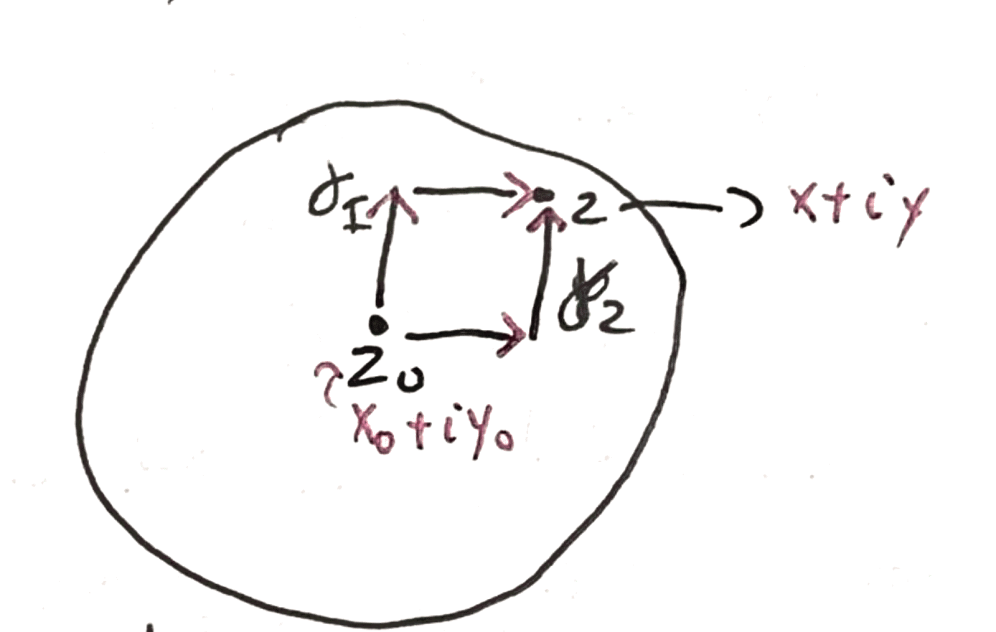
\includegraphics[width=.5\textwidth]{disk5.png}}\]
    For all $z \in \Omega$, define $F(z) = \int_{z_0}^z f(\xi) d\xi \coloneqq \int_{\gamma_1} f(z) dz = \int_{\gamma_2} f(z) dz$. We note that $F(z)$ is well-defined as Cauchy's Theorem guarantees the path-independence.\\\\
    \underline{We claim that $F \in CR^1(\Omega)$.} Indeed, tracing $\gamma_1$ and using the Fundamental Theorem of Calculus tells us that
    \[\frac{\partial F}{\partial x}(z) = f(z)\]
    Similarly, tracing along $\gamma_2$, we can parameterize $F(z)$ as
    \[F(z) = \int_{x_0}^x f(s + i y_0) ds + i \int_{y_0}^y f(x + it) dt\]
    Then it follows again that
    \[\frac{\partial F}{\partial y}(z) = i f(z)\]
    We can check that
    \[\frac{\partial F}{\partial x} + i \frac{\partial F}{\partial y} = f(z) - f(z) = 0\]
    , thus $F(z) \in CR^1(\Omega)$. Since $F(z)$ follows the Cauchy-Riemann Equations, we also know that
    \[F'(z) = \frac{1}{2}(\frac{\partial F}{\partial x} - i \frac{\partial F}{\partial y}) = \frac{1}{2}(2f(z)) = f(z)\]
    Since $F(z)$ is holomorphic, it is infinitely differentiable, so $f(z)$ is also holomorphic, so we are done.
\end{proof}

\begin{corollary}
    If $f_n \in C_z^1(\Omega)$ and $\{f_n\}$ converges to $f$ uniformly, then $f \in C_z^1(\Omega)$.
\end{corollary}

\begin{proof}
    For all sufficiently small rectangle $R$ within $\Omega$, consider
    \begin{align*}
        \int_{\partial R} f(z) dz &= \int_{\partial R} \lim_{n \to \infty} f_n dz\\
        &= \lim_{n \to \infty} \int_{\partial R} f_n dz \tag*{Uniform Convergence}\\
        &= \lim_{n \to \infty} 0 \tag*{Cauchy's Theorem}\\
        &= 0
    \end{align*}
    Thus, by Morera's Theorem, $f \in C_z^1(\Omega)$.
\end{proof}

\begin{corollary}
    If $f_n \in C_z^1(\Omega)$ and $\{f_n\}$ converges to $f$ uniformly, then $\{f_n'(z)\}$ converges to $f'(z)$ uniformly, and hence $\{f_n^{k}(z)\}$ converges to $f^{k}(z)$ uniformly.
\end{corollary}

\begin{proof}
It suffices for us to show this for the first derivative. Now for all $z \in \Omega$ and sufficiently small domain $G$, we have that
\begin{align*}
    f'(z) &= \frac{1}{2 \pi i} \int_{\partial G} \frac{f(z)}{(\xi - z)^2} d\xi \tag*{Cauchy's Formula for Derivatives}\\
    &= \frac{1}{2 \pi i} \int_{\partial G} \lim_{n \to \infty} \frac{f_n(z)}{(\xi - z)^2} d\xi\\
    &= \lim_{n \to \infty} \frac{1}{2 \pi i} \int_{\partial G} \frac{f_n(z)}{(\xi - z)^2} d\xi \tag*{Uniform Convergence}\\
    &= \lim_{n \to \infty} f_n'(z) \tag*{Cauchy's Formula for Derivatives}
\end{align*}
Thus, we have that $\{f_n'(z)\}$ converges to $f'(z)$. Since the original convergence is uniform, this convergence is also uniform.
\end{proof}

\begin{theorem}[Meta Theorem]
    Let $\phi(z, \xi): \Cbb \times X \to \Cbb$ where $X$ is some parameterization space with measure $\mu(\xi)$ that is finite, let
    $$f(z) = \int \phi(z, \xi) d\mu(\xi)$$
    Suppose $\phi$ is $CR^1$ in the variable $z$ and $f$ is bounded, then $f(z)$ is analytic.
\end{theorem}

\begin{proof}
    Since the measure $\mu$ is finite and the function is bounded, we can use Fubini's Theorem and see that, for all sufficiently small rectangles,
    \begin{align*}
        \int_R f(z) dz &= \int_R [\int \phi(z, \xi) d\mu(\xi)] dz\\
        &= \int [\int_R \phi(z, \xi) dz] d\mu(\xi) \tag*{Fubini's Theorem}\\
        &= \int 0 d\mu(\xi) \tag*{$\phi$ is $CR^1$ in the variable $z$}\\
        &= 0
    \end{align*}
\end{proof}

\begin{corollary}
    Let $f(z) = \sum_{n = 0}^\infty a_n (z - z_0)^n$ defined in $D_{z_0, r}$, then $f \in CR^1(D_{z_0, r}) = C_z^1(D_{z_0, r})$
\end{corollary}

\begin{proof}
    Let $z \in D(z_0, r)$, consider $r_1 > 0$ small enough that $cl(D(z, r_1)) \subset D(z_0, r)$, then by Heine-Cantor, we know that the partial sums
    \[\sum_{k = 0}^N a_k (z - z_0)^k \mapsto \sum_{0}^\infty a_n (z - z_0)^n \text{ converges uniformly in $D(z, r_1)$}\]
    Each of the partial sum are complex differentiable, thus by Corollary above, we have that $f \in C_z^1(D_{z_0, r})$.
\end{proof}

\begin{theorem}
    $CR^1 = C_z^1 = \text{Analytic}$
\end{theorem}

\begin{proof}
We have already shown all the directions in previous lectures and this lecture.
\end{proof}

\subsection{Power Series}

\begin{definition}
    Let $f(z) = \sum a_k (z - z_0)^k$ be a power series. We define the radius of convergence of $f$ as $R \in [0, \infty]$ such that for all $z$ such that $|z - z_0| < R$, $f(z)$ diverges, and for all $z$ such that $|z - z_0| > R$, $f(z)$ converges.
\end{definition}

\begin{remark}
    It turns out that
    \[\frac{1}{R} \coloneqq \lim \sup_{n \to \infty} |a_n|^{1/n}\]
\end{remark}

\begin{proposition}
    Let $f(z) = \sum a_k (z - z_0)^k$ be a power series with radius of convergence $R$, then $f(z)$ converges uniformly in any smaller disk of radius $r < R$ contained in $D_{z_0, R}$
\end{proposition}

\begin{proof}
    We note that $f$ is continuous on $D_{z_0, R}$, and the closure of any smaller disk is also contained in $D_{z_0, R}$, then apply Heine-Cantor.
\end{proof}

\begin{corollary}
    The following three power series:
    \begin{itemize}
        \item $\sum_{n = 0}^\infty a_n z^n$
        \item $\sum_{n = 0}^\infty n a_n z^{n-1}$
        \item $\sum_{n = 0}^\infty \frac{a_n}{n + 1} z^{n+1}$
    \end{itemize}
    all have the same radius of convergence.
\end{corollary}

\begin{proof}
    Exercise. Hint: Note that
    \[\lim_{n \to \infty} n^{1/n} = 1\]
\end{proof}

\begin{example}
    For sufficiently small $z \in \Cbb$, consider
    \[\frac{1}{1 + sin(z)} = 1 - sin(z) + sin^2(z) + ...\]
    , we can rewrite this into a power-series by noting that
    \[sin(z) = z - \frac{z^3}{3!} + \frac{z^5}{5!} + ...\]
\end{example}

\subsection{Liouville's Theorem}

\begin{theorem}
    Let $f \in Hol(\Cbb)$ be a holomorphic function on $\Cbb$, and for all $z \in \Cbb$ we have that $|f(z)| \leq M$ for some fixed $M \in \Cbb$, then $f(z)$ is identically constant.
\end{theorem}

\begin{proof}
Using Cauchy's Formula for Derivatives, we note that for all $z \in \Cbb$, for all $R > 0$,
\[f'(z) = \frac{1}{2\pi i} \int_{|\xi - z| = R} \frac{f(\xi)}{(\xi - z)^2} d\xi\]
Thus, we have that
\begin{align*}
    |f'(z)| \leq \frac{1}{2\pi} \max_{\xi \in |\xi - z|} |\frac{f(\xi)}{(\xi - z)^2}| \cdot 2 \pi R\\
    &\leq \frac{1}{2\pi} \frac{M}{R^2} \cdot 2 \pi R \tag*{Since $f$ is bounded}\\
    &= \frac{M}{R}
\end{align*}
Since this inequality holds for all $R > 0$, taking the limit as $R \to 0$, gives us that
\[|f'(z)| = 0\]
Hence $f'(z) = 0$, so
\[\frac{\partial f}{\partial z} = 0, \frac{\partial f}{\partial \overline{z}} = 0\]
So in other words
\[f_x - i f_y = 0, f_x + i f_y = 0 \implies f_x = 0, f_y = 0 \implies f(z) \text{ is constant}\]
\end{proof}

\begin{remark}
    While our Morera's Theorem applies to only triangles, up to a change of coordinate, the rectangle can really just be anything.
\end{remark}

\begin{remark}
    How to check say if $f(z) = |z|^2 = z \overline{z}$ is analytic or not? Well, we see that
    \[\frac{\partial f}{\partial \overline{z}} = \frac{\partial z}{\partial \overline{z}} \overline{z} + z \frac{\partial \overline{z}}{\partial \overline{z}} = 0 + z(1) \neq 0\]
    Thus, $f$ is not holomorphic and hence not analytic.\\\\
    Take another example, say $f(z) = |z| = (z \overline{z})^{1/2}$. This is real valued so we can use power rule and
    \[\overline{\partial}(f) = \frac{1}{2}(z \overline{z})^{-1/2} z \neq 0\]
\end{remark}

\newpage

\section{Lecture 6}




\end{document}
